% kidbox: An Architectural Field Guide
% A deep-dive technical report on how the kidbox project works and is configured,
% with generous tangents into the technologies it touches (and a few it does not).
%
% Build:  pdflatex kidbox-architecture.tex   (run twice for the table of contents)

\documentclass[11pt,oneside]{article}

% ---------------------------------------------------------------------------
% Page geometry
% ---------------------------------------------------------------------------
\usepackage[T1]{fontenc}
\usepackage[utf8]{inputenc}
\usepackage[margin=0.75in]{geometry}
\setlength{\headheight}{14pt}

% ---------------------------------------------------------------------------
% Fonts: Charter for the body (very readable for long-form reading),
% Helvetica for headings, Computer Modern Typewriter for code.
% ---------------------------------------------------------------------------
\usepackage{lmodern}   % provides a bold typewriter; charter/helvet override rm & sf below
\usepackage{charter}
\usepackage[scaled=0.90]{helvet}
\usepackage{microtype}
\emergencystretch=3em   % absorb the occasional long, unbreakable file path

% ---------------------------------------------------------------------------
% Colour palette
% ---------------------------------------------------------------------------
\usepackage{xcolor}
\definecolor{ink}{HTML}{1A2230}        % near-black body text
\definecolor{kbblue}{HTML}{1F4E79}     % primary
\definecolor{kbteal}{HTML}{0E7C86}     % accent
\definecolor{kbamber}{HTML}{B26A00}    % warnings / rough edges
\definecolor{kbgreen}{HTML}{2F6F4F}    % "try this"
\definecolor{kbgrey}{HTML}{5B6472}
\definecolor{codebg}{HTML}{F6F7F9}
\definecolor{codeframe}{HTML}{D9DEE6}
\definecolor{rulegrey}{HTML}{C8CFDA}
\definecolor{kw}{HTML}{1F4E79}
\definecolor{str}{HTML}{0E7C86}
\definecolor{cmt}{HTML}{7A8595}

\color{ink}

% ---------------------------------------------------------------------------
% Spacing
% ---------------------------------------------------------------------------
\usepackage{parskip}
\usepackage{enumitem}
\setlist{itemsep=2pt,topsep=4pt,parsep=0pt}
\usepackage{booktabs}
\usepackage{array}

% ---------------------------------------------------------------------------
% Section styling
% ---------------------------------------------------------------------------
\usepackage{titlesec}
\titleformat{\section}
  {\normalfont\sffamily\Large\bfseries\color{kbblue}}
  {\thesection}{0.7em}{}[{\color{rulegrey}\titlerule[1pt]}]
\titleformat{\subsection}
  {\normalfont\sffamily\large\bfseries\color{ink}}
  {\thesubsection}{0.6em}{}
\titleformat{\subsubsection}
  {\normalfont\sffamily\normalsize\bfseries\color{kbteal}}
  {\thesubsubsection}{0.5em}{}
\titlespacing*{\section}{0pt}{1.6\baselineskip}{0.5\baselineskip}

% ---------------------------------------------------------------------------
% Headers / footers
% ---------------------------------------------------------------------------
\usepackage{fancyhdr}
\pagestyle{fancy}
\fancyhf{}
\renewcommand{\headrulewidth}{0.4pt}
\renewcommand{\headrule}{\hbox to\headwidth{\color{rulegrey}\leaders\hrule height \headrulewidth\hfill}}
\fancyhead[L]{\footnotesize\sffamily\color{kbgrey}kidbox}
\fancyhead[R]{\footnotesize\sffamily\color{kbgrey}\leftmark}
\fancyfoot[C]{\footnotesize\sffamily\color{kbgrey}\thepage}

% ---------------------------------------------------------------------------
% Code listings
% ---------------------------------------------------------------------------
\usepackage{listings}
\lstdefinestyle{kb}{
  backgroundcolor=\color{codebg},
  basicstyle=\ttfamily\footnotesize\color{ink},
  keywordstyle=\color{kw},
  commentstyle=\color{cmt}\itshape,
  stringstyle=\color{str},
  numberstyle=\tiny\color{kbgrey},
  frame=single,
  rulecolor=\color{codeframe},
  framesep=6pt,
  xleftmargin=10pt,
  xrightmargin=4pt,
  breaklines=true,
  breakatwhitespace=true,
  showstringspaces=false,
  columns=fullflexible,
  keepspaces=true,
  upquote=true,
  aboveskip=10pt,
  belowskip=6pt,
}
\lstset{style=kb}
\newcommand{\code}[1]{\texorpdfstring{\textcolor{kbblue}{\texttt{#1}}}{#1}}
\newcommand{\file}[1]{\textcolor{kbteal}{\texttt{#1}}}

% ---------------------------------------------------------------------------
% Callout boxes
% ---------------------------------------------------------------------------
\usepackage[most]{tcolorbox}

\newtcolorbox{deeper}[1][Going deeper]{
  enhanced, breakable, colback=kbblue!4, colframe=kbblue,
  boxrule=0.4pt, left=10pt, right=10pt, top=8pt, bottom=8pt,
  arc=2pt, fonttitle=\sffamily\bfseries\small\color{white},
  coltitle=white, title={#1},
  attach boxed title to top left={xshift=8pt,yshift=-\tcboxedtitleheight/2},
  boxed title style={colback=kbblue,arc=1pt,boxrule=0pt}
}
\newtcolorbox{fieldnote}[1][Field note]{
  enhanced, breakable, colback=kbamber!6, colframe=kbamber,
  boxrule=0.4pt, left=10pt, right=10pt, top=8pt, bottom=8pt,
  arc=2pt, fonttitle=\sffamily\bfseries\small\color{white},
  coltitle=white, title={#1},
  attach boxed title to top left={xshift=8pt,yshift=-\tcboxedtitleheight/2},
  boxed title style={colback=kbamber,arc=1pt,boxrule=0pt}
}
\newtcolorbox{tryit}[1][Try this]{
  enhanced, breakable, colback=kbgreen!5, colframe=kbgreen,
  boxrule=0.4pt, left=10pt, right=10pt, top=8pt, bottom=8pt,
  arc=2pt, fonttitle=\sffamily\bfseries\small\color{white},
  coltitle=white, title={#1},
  attach boxed title to top left={xshift=8pt,yshift=-\tcboxedtitleheight/2},
  boxed title style={colback=kbgreen,arc=1pt,boxrule=0pt}
}

% ---------------------------------------------------------------------------
% Diagrams
% ---------------------------------------------------------------------------
\usepackage{tikz}
\usetikzlibrary{arrows.meta,positioning,calc,shadows.blur,fit,backgrounds}
\tikzset{
  stage/.style={draw=kbblue,fill=kbblue!6,rounded corners=2pt,
    font=\sffamily\small,align=center,inner sep=6pt,minimum height=9mm},
  accent/.style={draw=kbteal,fill=kbteal!8,rounded corners=2pt,
    font=\sffamily\small,align=center,inner sep=6pt,minimum height=9mm},
  flow/.style={-{Latex[length=2.4mm]},draw=kbgrey,thick},
  lbl/.style={font=\sffamily\scriptsize\itshape,color=kbgrey},
}

% ---------------------------------------------------------------------------
% Hyperlinks
% ---------------------------------------------------------------------------
\usepackage[hidelinks]{hyperref}
\hypersetup{
  colorlinks=true, linkcolor=kbblue, urlcolor=kbteal, citecolor=kbteal,
  pdftitle={kidbox: An Architectural Field Guide},
  pdfauthor={Prepared for Robert Utterback},
}

\setcounter{tocdepth}{2}
\setcounter{secnumdepth}{2}

% A small heading typeface helper
\newcommand{\sff}[1]{{\sffamily #1}}

\begin{document}

% ===========================================================================
% Title page
% ===========================================================================
\begin{titlepage}
\thispagestyle{empty}
\begin{center}
\vspace*{1.2cm}
{\color{rulegrey}\rule{\textwidth}{1.2pt}}\\[1.0em]
{\sffamily\bfseries\Huge\color{kbblue} kidbox}\\[0.45em]
{\sffamily\LARGE\color{ink} An Architectural Field Guide}\\[0.8em]
{\sffamily\large\color{kbgrey} How a locked-down, retro kid-computer is built\\
out of a stack of small, explicit Unix parts}\\[0.9em]
{\color{rulegrey}\rule{\textwidth}{1.2pt}}
\end{center}

\vfill

\begin{center}
\begin{minipage}{0.86\textwidth}
\small\itshape\color{kbgrey}
A deep but companionable tour of the boot chain, the console, the X Window
System, systemd, the input subsystem, the power button, and the typesetting
of the instruction booklet --- with frequent detours into how these
technologies came to be, and into roads the project chose \emph{not} to take.
Written to be printed, folded under one arm, and read in bed.
\end{minipage}
\end{center}

\vfill

\begin{center}
\small\sffamily\color{kbgrey}
Prepared for Robert Utterback \quad$\cdot$\quad Repository: \texttt{robertutterback/kidbox}\\[0.3em]
Technical report \quad$\cdot$\quad \today
\end{center}
\end{titlepage}

% ===========================================================================
\tableofcontents
\thispagestyle{empty}
\clearpage

% ===========================================================================
\section{How to read this report}

This document explains, in more detail than is strictly necessary, how the
\textbf{kidbox} project turns a Raspberry Pi into a deliberately simple
computer for two children. You asked for something detailed yet interesting:
a piece of professional development you can enjoy rather than endure. So
alongside the literal description of what each file does, there are three
kinds of marginal excursion you will see throughout:

\begin{deeper}
A \textbf{Going deeper} box steps back from kidbox itself to explain the
technology underneath --- where it came from, why it works the way it does,
and what else it can do. These are the parts that are fun to know even though
the project would run fine if you never read them.
\end{deeper}

\begin{tryit}
A \textbf{Try this} box suggests a harmless experiment you can run on the Pi
(or any Linux box) to see a concept with your own eyes. None of them are
required reading.
\end{tryit}

\begin{fieldnote}
A \textbf{Field note} flags something I noticed while reading the code: a
latent bug, a rough edge, a place where the comments and the behaviour have
drifted apart. You said you vibe-coded most of this and fix the ``AI slop''
yourself, so these are offered in that spirit --- small observations, not
criticisms.
\end{fieldnote}

The big idea of kidbox, stated in its own README, is worth keeping in mind the
whole way through:

\begin{quote}\itshape
``Intentionally simple and explicit. The idea is that the only way to use such
a computer is to start understanding how it works.''
\end{quote}

That philosophy is not just a slogan about the \emph{child's} experience. It
also describes the \emph{engineering}: kidbox is assembled from many small,
old, well-understood Unix tools, each doing one visible thing, wired together
with shell scripts you can read in an afternoon. There is no framework, no
container, no daemon you can't \texttt{cat}. That makes it an unusually good
specimen for a guided dissection.

% ===========================================================================
\section{The shape of the whole system}

Before the details, here is the system in one breath. A Raspberry Pi powers
on, boots Linux, and \emph{automatically logs in} a passwordless user named
\texttt{girls} on the first virtual terminal. That user's login shell runs a
snippet that enlarges the console font and launches a text menu drawn by
\texttt{whiptail}. The menu is the entire user interface. When a child picks an
activity, the menu starts a \emph{throwaway} graphical X session containing
exactly one program --- Tux Paint, say, or the Logo turtle --- and nothing
else: no desktop, no taskbar, no way out except finishing. When the program
quits, X is torn down and the child is back at the menu. A background service
watches the physical power button so that a careless poke shows a confirmation
dialog instead of yanking the power.

Everything kidbox adds to a stock Raspberry Pi OS falls into a few buckets:

\begin{itemize}
\item \textbf{A user and its login wiring} --- the \texttt{girls} account, console
autologin, a font, and a menu launched from \file{.bash\_profile}.
\item \textbf{A menu} --- one \texttt{bash} script (\file{menu.sh}) using
\texttt{whiptail} for the list and a helper to launch X programs.
\item \textbf{On-demand X sessions} --- \texttt{xinit} plus a tiny
\file{.xinitrc} that starts a minimal window manager and one application.
\item \textbf{A handful of activities} --- two are ordinary desktop programs
(Tux Paint, Leafpad), three are vintage programming environments (UCBLogo,
PC-BASIC), and three are home-grown (an HTML clock, a shell timer, a shell
stopwatch).
\item \textbf{Power-button safety} --- a \texttt{systemd-logind} tweak plus a
small Python service reading the kernel's input devices.
\item \textbf{An instruction booklet} --- a LaTeX document typeset and imposed
for saddle-stitch printing.
\end{itemize}

Figure~\ref{fig:overview} shows how the pieces relate.

\begin{figure}[ht]
\centering
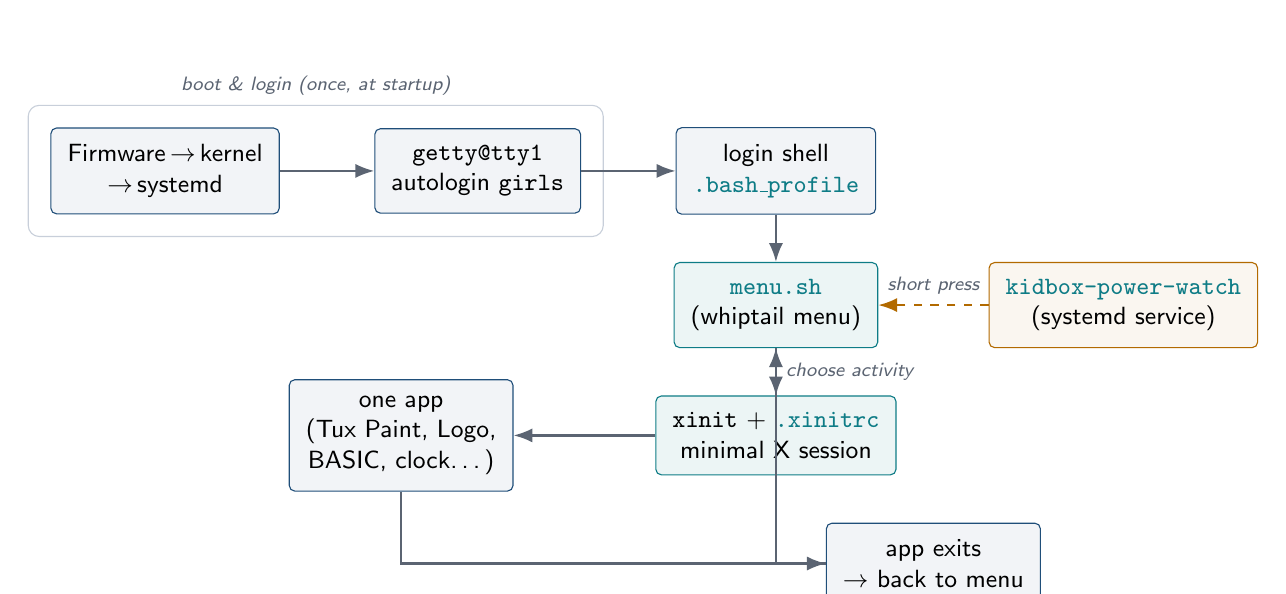
\begin{tikzpicture}[node distance=6mm and 12mm]
\node[stage] (boot) {Firmware\,$\to$\,kernel\\$\to$\,systemd};
\node[stage,right=of boot] (getty) {\texttt{getty@tty1}\\autologin \texttt{girls}};
\node[stage,right=of getty] (shell) {login shell\\\file{.bash\_profile}};
\node[accent,below=of shell] (menu) {\file{menu.sh}\\(whiptail menu)};
\node[accent,below=of menu] (xinit) {\texttt{xinit} + \file{.xinitrc}\\minimal X session};
\node[stage,left=18mm of xinit] (app) {one app\\(Tux Paint, Logo,\\BASIC, clock\dots)};
\node[stage,below=of xinit,xshift=20mm] (back) {app exits\\$\to$ back to menu};

\node[fit=(boot)(getty),draw=rulegrey,rounded corners,inner sep=8pt,
  label={[lbl]above:boot \& login (once, at startup)}] {};

\draw[flow] (boot)--(getty);
\draw[flow] (getty)--(shell);
\draw[flow] (shell)--(menu);
\draw[flow] (menu)--node[lbl,right]{choose activity}(xinit);
\draw[flow] (xinit)--(app);
\draw[flow] (app) |- (back);
\draw[flow] (back) -| (menu);

% power watcher, off to the side
\node[draw=kbamber,fill=kbamber!6,rounded corners=2pt,font=\sffamily\small,
  align=center,inner sep=6pt,right=14mm of menu] (pwr)
  {\file{kidbox-power-watch}\\(systemd service)};
\draw[flow,dashed,draw=kbamber] (pwr)--node[lbl,above,align=center]{short press}(menu);
\end{tikzpicture}
\caption{The life of the machine. Boot and login happen once; the
menu\,$\to$\,app\,$\to$\,menu loop runs forever. The power watcher sits to the
side, waking only when the button is pressed.}
\label{fig:overview}
\end{figure}

\begin{deeper}[Going deeper: why ``one program, then throw it away''?]
Most computers run a \emph{session}: a desktop that persists, with many windows
and a way to switch between them. kidbox deliberately refuses this. Each
activity gets a fresh, single-window X server that exists only for the lifetime
of that one program. This is the same trick a \emph{kiosk} uses --- an airport
check-in screen, a museum exhibit --- and it buys three things at once:
\emph{isolation} (a crash takes down only that activity), \emph{simplicity}
(there is no window management to learn or escape), and \emph{statelessness}
(every activity starts clean). The cost is start-up latency: spinning up an X
server takes a second or two. For a child choosing one thing at a time, that
trade is clearly worth it.
\end{deeper}

% ===========================================================================
\section{From power-on to a menu: the boot and login chain}

This is the most ``Linux internals'' part of the project, and the part you said
you'd not had to configure before. Let's walk the whole chain.

\subsection{Firmware, kernel, and the hand-off to \texttt{init}}

When a Raspberry Pi powers on, its \emph{firmware} (on the Pi, code running on
the VideoCore GPU, not a traditional PC BIOS/UEFI) reads the boot partition,
loads the Linux kernel, and jumps into it. The kernel brings up hardware,
mounts the root filesystem, and then starts exactly one user-space process,
historically called \texttt{init}, with process ID~1. On Raspberry Pi OS (a
Debian derivative) that process is \textbf{systemd}.

systemd's job is to bring the system up to a \emph{target} --- a named
collection of services that should be running. kidbox cares about
\texttt{multi-user.target} (a fully booted, networked, text-mode system) rather
than \texttt{graphical.target} (which would start a graphical login manager).
kidbox never installs a graphical login manager, so the machine naturally rests
at the multi-user, text-console state. That is the foundation the whole design
rests on: \textbf{boot to a console, not to a desktop.}

\begin{deeper}[Going deeper: targets, and the ghost of runlevels]
If you came up on older Unix or Linux, you remember \emph{runlevels}: a single
number (0--6) describing how much of the system was running, set in
\file{/etc/inittab}. Runlevel 3 was ``multi-user text mode,'' runlevel 5 added
graphics, runlevel 0 was halt, 6 was reboot. systemd replaced this with
\emph{targets}, which are just units that depend on other units, so the model
is a graph rather than a ladder. The old names survive as compatibility
aliases: \texttt{runlevel3.target} \emph{is} \texttt{multi-user.target}. You can
ask the running system what it's aiming for with \texttt{systemctl
get-default}, and where it is right now with \texttt{systemctl
list-units -{}-type target}.
\end{deeper}

\subsection{\texttt{getty}, \texttt{agetty}, and automatic login}

A text console is offered to you by a program called a \textbf{getty}. The name
is a fossil: it stands for ``get tty,'' and a \emph{tty} is in turn short for
\emph{teletypewriter} --- the electromechanical printing terminals that were the
first interactive Unix consoles in the early 1970s. The getty's classic job was
to watch a terminal line, print the \texttt{login:} prompt, read a username, and
hand off to the \texttt{login} program to check the password.

On a systemd machine each text console is managed by a templated service,
\texttt{getty@.service}, instantiated per virtual terminal: \texttt{getty@tty1},
\texttt{getty@tty2}, and so on. The actual program run is \texttt{agetty}
(``alternative getty''). kidbox needs the first console to skip the
username/password dance and log the \texttt{girls} user straight in. The README
does this with a systemd \emph{drop-in} override:

\begin{lstlisting}[language=bash]
sudo systemctl edit getty@tty1
\end{lstlisting}

\begin{lstlisting}
[Service]
ExecStart=
ExecStart=-/sbin/agetty --autologin girls --noclear %I $TERM
\end{lstlisting}

Two subtleties hide in those four lines, and they're worth understanding
because they trip up nearly everyone the first time:

\begin{itemize}
\item The \textbf{empty \code{ExecStart=}}. A systemd service may normally have
only one \texttt{ExecStart}. The packaged \texttt{getty@.service} already
defines one. Assigning an empty value first \emph{clears} the inherited command,
and the second line sets the replacement. Without the blank line you'd get an
error about multiple \texttt{ExecStart} directives.
\item The \textbf{leading dash} in \code{-/sbin/agetty}. In a systemd unit a
dash before the executable means ``a non-zero exit from this process is not a
failure.'' Gettys come and go constantly as people log in and out; the dash
keeps systemd from treating a normal exit as a fault.
\end{itemize}

\code{--autologin girls} tells \texttt{agetty} to bypass authentication and run
\texttt{login} for that user directly. \code{--noclear} stops it from clearing
the screen first. \code{\%I} is the instance name (here \texttt{tty1}), and
\code{\$TERM} carries the terminal type.

\begin{fieldnote}
The README adds a wise warning: don't use \texttt{raspi-config}'s autologin
option, because that wires autologin to \emph{your} user (the \texttt{pi}-style
admin account), not to \texttt{girls}. Doing this by hand is the correct call.
The only thing missing is a reminder that \texttt{systemctl edit} writes to
\file{/etc/systemd/system/getty@tty1.service.d/override.conf} and that you can
inspect the merged result with \texttt{systemctl cat getty@tty1} --- handy when
it mysteriously doesn't take effect.
\end{fieldnote}

\begin{deeper}[Going deeper: the virtual terminals behind Ctrl+Alt+F1]
The Linux kernel multiplexes one physical screen and keyboard into a dozen
independent text consoles, the \emph{virtual terminals} (VTs). You switch
between them with Ctrl+Alt+F1 through F6 (and beyond). Each is a fully separate
login session. kidbox leans on this hard: the child's menu lives on
\texttt{tty1}, and --- as we'll see --- the power-button confirmation dialog
deliberately pops up on \texttt{tty12}, an otherwise-unused VT, so the two never
fight over the keyboard. The current VT is readable at any time from
\file{/sys/class/tty/tty0/active}, and you can switch programmatically with the
\texttt{chvt} command. This is one of those Linux facilities that feels archaic
until you need exactly it, at which point it is perfect.
\end{deeper}

\subsection{Login shells, and why the menu lives in \file{.bash\_profile}}

Once \texttt{login} succeeds, it starts the user's \emph{login shell} ---
\texttt{bash}. Here we meet a distinction that confuses almost everyone:

\begin{itemize}
\item A \textbf{login shell} (what you get from console login, autologin, or
\texttt{ssh}) reads \file{/etc/profile} and then the first it finds of
\file{\textasciitilde/.bash\_profile}, \file{\textasciitilde/.bash\_login}, or
\file{\textasciitilde/.profile}.
\item An \textbf{interactive non-login shell} (a new terminal window inside an
already-running desktop) reads \file{\textasciitilde/.bashrc} instead.
\end{itemize}

kidbox wants its menu to appear \emph{exactly once, at the moment of login}, so
the autostart logic belongs in \file{.bash\_profile} --- and that is precisely
where the installer puts it. The snippet (\file{config/bash\_profile\_snippet.sh})
is short and careful:

\begin{lstlisting}[language=bash]
# Auto-run kid menu only on local interactive TTY (not SSH)
if [[ -t 0 && -z "${SSH_CONNECTION:-}" ]]; then
  if command -v setfont >/dev/null 2>&1; then
    (setfont ter-v32n || setfont ter-132n \
       || setfont /usr/share/consolefonts/Lat15-Terminus32x16.psf.gz) \
       >/dev/null 2>&1 || true
  fi
  setterm --blank 10 2>/dev/null || true
  "$HOME/bin/menu.sh"
fi
\end{lstlisting}

The guard \code{[[ -t 0 \&\& -z "\$\{SSH\_CONNECTION:-\}" ]]} is the clever bit.
\code{-t 0} asks ``is standard input a terminal?'' (true on a real console,
false if a script piped input in). \code{-z "\$\{SSH\_CONNECTION:-\}"} asks
``is the \texttt{SSH\_CONNECTION} variable empty?'' --- it is set automatically by
\texttt{sshd} for remote logins. Together they mean: \emph{only launch the
kiosk menu when someone is physically at the machine.} If you SSH in to fix
something, you get a normal shell, not the locked-down menu. That single line is
the maintenance escape hatch for the whole appliance.

\begin{tryit}
On any Linux box, run \texttt{echo \$SSH\_CONNECTION} in an SSH session and then
again on the physical console. Remote, it prints four numbers (client IP, client
port, server IP, server port); local, it prints an empty line. That's the exact
signal kidbox uses to tell ``here'' from ``there.''
\end{tryit}

\subsection{Making the console legible: console fonts and blanking}

Two more things happen before the menu appears, both aimed at small children
reading a screen from across a desk.

\textbf{The font.} \code{setfont ter-v32n} loads a Terminus console font that is
32 pixels tall --- roughly double the default. The cascade of fallbacks
(\code{ter-132n}, then an explicit path) is defensive: different Debian releases
name and ship these fonts slightly differently, so the snippet tries three
spellings and shrugs off failure with \code{|| true}. \texttt{setfont} comes
from the \texttt{kbd} package, which the installer dutifully lists.

\textbf{The blanking.} \code{setterm --blank 10} tells the kernel console to go
dark after 10 minutes of inactivity --- a crude screensaver for the text mode,
distinct from the X-level blanking we'll meet later.

\begin{deeper}[Going deeper: what a console font actually \emph{is}]
A graphical desktop renders text from scalable outline fonts (TrueType,
OpenType) at any size. The Linux \emph{text} console predates all that: it draws
characters from a fixed bitmap \emph{glyph table} called a PSF file (``PC Screen
Font''). A PSF is almost comically simple --- a tiny header, then one bitmap per
glyph, each glyph a fixed grid of pixels (Terminus 32$\times$16 means each
character is 16 px wide and 32 px tall) --- plus an optional Unicode mapping
table that says which code points each glyph represents. Because the glyphs are
fixed-size bitmaps, ``making the font bigger'' on the console doesn't mean
scaling; it means \emph{loading a different file with taller glyphs}, which is
exactly what \texttt{setfont ter-v32n} does. The \texttt{console-setup} package
(also installed by kidbox) is the mechanism for making such a choice
\emph{persist} across reboots, by regenerating the font at boot; the
\file{.bash\_profile} approach instead sets it freshly at each login, which is
simpler and good enough here.
\end{deeper}

% ===========================================================================
\section{The menu: \texttt{whiptail}, \texttt{newt}, and a button that hides}

The menu is the heart of kidbox and a tidy little study in old-school terminal
UI. It lives in \file{bin/menu.sh}. Structurally it is an infinite
\code{while true} loop: draw a menu, read the choice, launch the chosen
activity, and when that returns, loop back and draw the menu again. The only way
out is the ``Shutdown'' item.

\subsection{Drawing a menu with \texttt{whiptail}}

\texttt{whiptail} draws text-mode dialog boxes --- menus, message boxes, input
prompts, progress bars --- using box-drawing characters and colour. kidbox uses
its \code{--menu} mode:

\begin{lstlisting}[language=bash]
CHOICE=$(
  whiptail --title "$MENU_TITLE" --nocancel \
    --menu "Choose something to do" "$TERM_LINES" "$TERM_COLS" "$MENU_ROWS" \
      "${MENU_ITEMS[@]}" \
    3>&1 1>&2 2>&3
)
\end{lstlisting}

Two pieces of arcana are worth unpacking.

\textbf{The \code{3>\&1 1>\&2 2>\&3} dance.} This is the single most
head-scratching idiom in terminal scripting. \texttt{whiptail} draws its
\emph{interface} on standard output but prints the user's \emph{selection} on
standard error --- precisely so the drawing and the result don't get mixed in a
pipe. But \code{\$(...)} captures standard output, not standard error. The
juggling swaps the two streams: open a temporary file descriptor 3 pointing at
the original stdout (the screen), send stdout to stderr, send stderr to fd~3.
Net effect: the menu still draws on the real screen, and the \emph{answer}
flows back through \code{\$(...)} into \code{CHOICE}. It looks like line noise;
it is actually a precise plumbing diagram.

\textbf{Sizing to the terminal.} The menu reads \code{LINES} and \code{COLUMNS}
(falling back to \texttt{tput lines}/\texttt{tput cols}) so the dialog fills the
whole screen rather than floating in a small box. \code{MENU\_ROWS} is the
terminal height minus a few lines of chrome.

\subsection{Hiding the ``OK'' button: the \texttt{NEWT\_COLORS} trick}

Here is my favourite hack in the whole repository, and the comments in the code
already explain the constraint honestly. \texttt{whiptail} can suppress its
\emph{Cancel} button with \code{--nocancel}, but it offers \emph{no} switch to
hide the \emph{OK} button. For a child-proof kiosk you don't want a focusable
``OK'' to tab to and wonder about. So the author makes the button
\emph{invisible by colouring it to match the background}:

\begin{lstlisting}[language=bash]
export NEWT_COLORS='
root=white,blue
window=white,blue
button=white,blue
actbutton=white,blue
...
'
\end{lstlisting}

Every element is white-on-blue, including both the resting and active button
colours, so the OK button is still \emph{there} and still works --- it has
simply been painted into the wallpaper. This is a wonderfully pragmatic piece of
``simple and explicit'' engineering: rather than patch \texttt{whiptail} or
switch toolkits, paint the unwanted control the colour of the wall.

\begin{deeper}[Going deeper: \texttt{whiptail} vs \texttt{dialog}, \texttt{newt} vs \texttt{ncurses}]
There are two great families of text-mode dialog tools, and they descend from
two different terminal libraries.

\texttt{whiptail} is built on \textbf{newt}, a library written at Red Hat in the
1990s; the name is a half-joke, ``Not Erik's Windowing Toolkit,'' after its
author's earlier ``Erik's Windowing Toolkit.'' newt is small, opinionated, and
drives its colours through the \texttt{NEWT\_COLORS} environment variable
kidbox exploits above.

The older, more featureful cousin is \texttt{dialog}, built on \textbf{ncurses}
--- the free reimplementation of AT\&T's \texttt{curses} library, which itself
grew out of the \texttt{vi} editor's need to move a cursor around any terminal
without caring what model it was. The magic underneath all of this is
\textbf{terminfo}: a database (\file{/usr/share/terminfo}) describing, for every
terminal type ever made, the exact byte sequences to move the cursor, clear the
screen, or turn text blue. When you set \code{TERM=linux} --- as the
power-button script explicitly does, because a systemd service has no inherited
terminal type --- you are choosing which page of that database curses/newt
should read. kidbox could have used \texttt{dialog} instead of \texttt{whiptail}
and the menu would look almost identical; \texttt{whiptail} wins here purely on
being tiny and already present on Raspberry Pi OS.
\end{deeper}

\subsection{Refusing to die: signal traps and the missing exit}

A kiosk must not be escapable by the usual ``break out of a program'' reflexes.
kidbox blocks the obvious one --- Ctrl+C --- with a single line near the top:

\begin{lstlisting}[language=bash]
if [[ "$DEV_MODE" == false ]]; then
  trap '' INT
fi
\end{lstlisting}

\code{trap '' INT} installs an \emph{empty} handler for \texttt{SIGINT}, the
signal Ctrl+C sends. An empty handler means ``catch it and do nothing,'' so
Ctrl+C at the menu is simply inert. The \code{--dev} flag leaves the trap off
(and adds an Exit option and lets Cancel quit) so you can iterate on a normal
laptop without trapping yourself in your own kiosk.

\begin{fieldnote}
A subtle, real consequence worth knowing: \code{trap '' INT} is \emph{inherited}
by child processes, so any program the menu launches \emph{in the same process
context} also ignores Ctrl+C. That's fine for the menu loop, but it's the reason
the timer/stopwatch instructions say ``Press Ctrl+C to stop'' yet run inside
their \emph{own} \texttt{xterm}, which gets a fresh signal disposition --- so
there the Ctrl+C does work. The two behaviours are consistent once you trace the
process tree, but it's the kind of thing that looks contradictory until you do.
\end{fieldnote}

There is also no ``Exit'' item in production mode, and pressing Esc (which
\texttt{whiptail} reports as a non-zero exit) hits the \code{continue} branch
that just redraws the menu. Between the trap, the missing exit, and the Esc
handling, there is no path from the menu back to a raw shell --- exactly the
intent.

% ===========================================================================
\section{Launching graphics on demand: the X Window System}

When the child picks Tux Paint or the Logo turtle, kidbox needs pixels, not
text. It gets them by starting a fresh, minimal \textbf{X} session around a
single program. This section is the densest in the report, because the X Window
System is a deep, 40-year-old piece of software and kidbox uses a surprising
amount of it deliberately.

\subsection{The \texttt{run\_x} helper and \texttt{xinit}}

The menu's launcher is a small function:

\begin{lstlisting}[language=bash]
run_x() {
  export KID_APP="$1"; shift || true
  export KID_ARGS="${*:-}"
  xinit -- :1 -br -nolisten tcp "vt${XDG_VTNR:-1}" >> "$LOGFILE" 2>&1
}
\end{lstlisting}

It records the chosen program in two environment variables, then calls
\texttt{xinit}. \texttt{xinit} is the bare-metal way to start X: it launches the
X \emph{server} and one \emph{client} (here, whatever \file{.xinitrc} runs), and
crucially, \textbf{when that client exits, \texttt{xinit} shuts the server
down.} That is the entire ``throwaway session'' mechanism --- no display
manager, no session daemon, just ``start X, run one thing, tear it all down.''

The arguments after \code{--} go to the X server:
\begin{itemize}
\item \code{:1} --- the \emph{display number}. X servers are addressed as
\code{:0}, \code{:1}, etc. kidbox uses \code{:1} to stay clear of any \code{:0}.
\item \code{-br} --- start with a black root window (no grey stipple flash).
\item \code{-nolisten tcp} --- do \emph{not} open a network port; accept only
local connections over a Unix socket. (More on why this matters below.)
\item \code{vt\$XDG\_VTNR} --- bind the server to the \emph{current} virtual
terminal, so graphics appear on the same screen the child is already looking at.
\code{XDG\_VTNR} is the VT number systemd exports for the session.
\end{itemize}

\begin{deeper}[Going deeper: what ``X'' actually is, and why it's a network protocol]
The X Window System (X11, 1987, out of MIT's Project Athena) is built on an idea
that still surprises people: it is a \textbf{client--server protocol}, and ---
counter-intuitively --- the \emph{server} is the thing in front of you. The X
\emph{server} owns the screen, keyboard, and mouse. Programs that want to draw
windows are \emph{clients}; they connect to the server and send requests like
``draw a line'' or ``tell me when a key is pressed.'' Because that conversation
is a network protocol, the client and server need not be on the same computer
--- this is how, decades before ``cloud,'' a Unix workstation could run a program
on a distant mainframe and display its windows locally. kidbox never wants that,
which is exactly why it passes \code{-nolisten tcp}: there is no reason to accept
connections from the network, so it refuses to even open the port, shrinking the
attack surface to zero. The clients on this machine reach the server through a
local Unix-domain socket instead. So a humble offline kid-computer quietly
demonstrates the most famous (and most debated) design decision in the history
of graphical Unix.
\end{deeper}

\subsection{Inside \file{.xinitrc}: a desktop in eleven lines}

When \texttt{xinit} starts the server, it runs the user's \file{.xinitrc} as the
session. kidbox's is about as small as a usable graphical environment gets:

\begin{lstlisting}[language=bash]
xset s on; xset s 600; xset +dpms; xset dpms 0 0 600   # blank after 10 min
[ -f ~/.Xresources ] && xrdb -merge ~/.Xresources       # load fonts/DPI
unclutter -idle 3 &                                     # hide idle cursor
matchbox-window-manager -use_titlebar no \
   -use_lowlight -use_fullscreen &                      # minimal WM
xbindkeys &                                             # global hotkeys
if [ -n "${KID_APP:-}" ]; then
  exec "$KID_APP" ${KID_ARGS:-}                         # become the app
fi
exec xterm                                              # fallback
\end{lstlisting}

Read it top to bottom and you have a complete, if spartan, desktop:

\begin{itemize}
\item \textbf{Screen blanking (\texttt{xset}).} \code{xset s 600} sets the
screensaver timeout to 600 seconds; \code{+dpms} enables DPMS (Display Power
Management Signaling), the standard by which the graphics card tells the monitor
to power down; \code{dpms 0 0 600} sets the standby/suspend/off timers so the
display actually sleeps after ten minutes. This is the X-session twin of the
console \code{setterm --blank} we saw earlier.
\item \textbf{Resources (\texttt{xrdb}).} \code{xrdb -merge ~/.Xresources} loads
the X resource database --- a key/value store of application preferences (fonts,
colours, DPI). More on this just below.
\item \textbf{Cursor hiding (\texttt{unclutter}).} Hides the mouse pointer after
3 idle seconds, so a forgotten cursor doesn't sit on the drawing.
\item \textbf{Window manager (\texttt{matchbox}).} A window manager decides
where windows go and draws their frames. \texttt{matchbox-window-manager} is a
minimalist WM designed for small/embedded screens; kidbox starts it with
\emph{no} title bars and \emph{fullscreen}, so the single app fills the display
with no decorations to poke at.
\item \textbf{Hotkeys (\texttt{xbindkeys}).} A daemon that binds key
combinations to commands, independent of which app has focus (see below).
\item \textbf{\code{exec} the app.} The script \emph{becomes} the chosen program
via \code{exec} (replacing the shell process). Because this is the last,
foreground client, \emph{its} exit is what tells \texttt{xinit} to bring the
whole server down --- closing the throwaway-session loop.
\end{itemize}

\begin{deeper}[Going deeper: the window manager is not the GUI]
Newcomers often assume ``the window manager'' \emph{is} the desktop. It isn't.
Under X, drawing windows is the application's job; the window manager only
decides \emph{where} top-level windows sit, draws their borders/title bars, and
handles moving, resizing, and focus. That separation is why you can swap
\texttt{matchbox} for \texttt{i3}, \texttt{openbox}, or a full GNOME shell
without changing a single application. kidbox exploits the separation to the
limit: by choosing the most minimal WM and turning off even its title bars, it
gets ``one fullscreen window, no chrome, nothing to manage'' --- a kiosk --- for
free. A fun corner case: you can legally run X with \emph{no} window manager at
all, in which case windows appear wherever the app asks and can't be moved.
\end{deeper}

\subsection{Big fonts everywhere: \texttt{.Xresources}, Xft, and DPI}

Children need large text, and X has two completely different font systems, both
of which kidbox touches in \file{config/Xresources}.

The modern path is \textbf{Xft} (the X FreeType interface), which renders
scalable, anti-aliased TrueType fonts. kidbox raises the global DPI so
everything scales up at once:

\begin{lstlisting}
Xft.dpi: 120
Xft.antialias: true
Xft.hintstyle: hintfull
XTerm*faceName: Monospace
XTerm*faceSize: 24
\end{lstlisting}

Setting \code{Xft.dpi} to 120 (from the usual 96) is a global ``make everything
\textsf{25\%} bigger'' lever for every Xft-aware app. The older path is the
original X core fonts, addressed by those intimidating strings:

\begin{lstlisting}
XTerm*font: -misc-fixed-medium-r-normal--20-200-75-75-c-100-iso10646-1
\end{lstlisting}

\begin{deeper}[Going deeper: decoding an XLFD, field by field]
That hyphen-salad is an \textbf{XLFD} --- an X Logical Font Description --- and it
is not random. It has fourteen fields, each delimited by a hyphen, describing one
specific bitmap font. Reading the example:

\smallskip
\begin{tabular}{@{}ll@{}}
\toprule
\textbf{Field} & \textbf{Value (meaning)}\\
\midrule
foundry        & \texttt{misc} (who made it)\\
family         & \texttt{fixed} (the typeface)\\
weight         & \texttt{medium} (vs.\ \texttt{bold})\\
slant          & \texttt{r} (roman; \texttt{i}=italic, \texttt{o}=oblique)\\
set width      & \texttt{normal}\\
pixel size     & \texttt{20} (glyph height in pixels)\\
point size     & \texttt{200} (deci-points, i.e.\ 20.0\,pt)\\
resolution x/y & \texttt{75}/\texttt{75} (DPI the font was designed for)\\
spacing        & \texttt{c} (character cell; \texttt{m}=monospace, \texttt{p}=proportional)\\
average width  & \texttt{100} (deci-pixels)\\
charset        & \texttt{iso10646-1} (Unicode)\\
\bottomrule
\end{tabular}
\smallskip

The wildcard \texttt{*} can stand in for any field, which is how people usually
write these (\texttt{-*-fixed-*-*-*-*-20-*-*-*-*-*-*-*}). kidbox spells out the
full description to pin down \emph{exactly} the 20-pixel fixed font it wants. The
fact that a project for two children contains a hand-written XLFD is a small
delight; almost nobody learns these any more.
\end{deeper}

\subsection{The one escape hatch: Ctrl+Alt+Backspace via \texttt{xbindkeys}}

There is exactly one intentional way to abandon a running activity, defined in
\file{config/xbindkeysrc}:

\begin{lstlisting}
"pkill -TERM Xorg"
  control+alt + BackSpace
\end{lstlisting}

Ctrl+Alt+Backspace runs \code{pkill -TERM Xorg}, which sends \texttt{SIGTERM} to
the X server. When the server dies, \texttt{xinit} returns, \code{run\_x}
returns, and the menu loop redraws --- so the child is safely back at the menu.

\begin{deeper}[Going deeper: ``zapping'' X, and why this keystroke is special]
Ctrl+Alt+Backspace is not an arbitrary choice. For most of X11's history it was
the built-in ``zap'' shortcut that instantly killed the X server --- a vital
panic button when a full-screen app wedged your machine. Around 2008,
distributions disabled it by default (too many people hit it by accident and
lost their work), moving it behind a keyboard option called
\texttt{terminate:ctrl\_alt\_bksp} or the server's \code{DontZapfrom} setting.
kidbox can't rely on that built-in being on, so it \emph{re-implements the
classic zap by hand} with \texttt{xbindkeys} and \texttt{pkill}. It's a lovely
historical echo: the project resurrects, in user space, a shortcut that was once
baked into the X server itself --- and uses it for exactly its original purpose,
a guaranteed way out.
\end{deeper}

% ===========================================================================
\section{The activities}

With the plumbing understood, the activities themselves are almost a victory
lap. There are eight menu items; they fall into three groups.

\subsection{Two ordinary desktop programs}

\textbf{Leafpad} (menu items 1--2) is a tiny GTK text editor, opened on a fixed
file per child --- \file{typing/sally.txt} or \file{typing/penny.txt}. The
installer is careful to create those files only if they don't already exist, so
a child's typing survives reinstalls (more on that in the install section).

\textbf{Tux Paint} (item 3) is a children's painting program from the early
2000s, complete with rubber-stamp clip art and sound effects. It needs no
configuration; kidbox just runs it fullscreen.

\subsection{Three vintage programming environments}

These are the soul of the project --- the ``start understanding how it works''
part made literal.

\textbf{UCBLogo} (item 4) is the turtle-graphics language. The menu opens it on
\file{logo/welcome.lg}, which defines a couple of procedures and draws a house
to greet the child.

\begin{deeper}[Going deeper: Logo, the turtle, and ``constructionism'']
Logo was created in 1967 at BBN by Wally Feurzeig, Cynthia Solomon, and Seymour
Papert. Papert --- who had worked with Jean Piaget --- believed children learn
deepest when \emph{building} things they care about, a philosophy he called
\emph{constructionism}. The ``turtle'' (originally a real floor robot dragging a
pen, later a screen cursor) lets a child \emph{become} the turtle: ``how would I
walk to draw a square?'' becomes \code{REPEAT 4 [FD 100 RT 90]}. Underneath the
playful syntax, Logo is a genuine dialect of \textbf{Lisp} --- lists are
first-class, procedures are values --- so a child doodling with the turtle is
quietly using one of computing's most profound language families. UCBLogo, the
implementation kidbox installs, was written by Brian Harvey at UC~Berkeley to
accompany his three-volume \emph{Computer Science Logo Style}.
\end{deeper}

\textbf{PC-BASIC} (item 5) is a faithful emulator of \textbf{GW-BASIC}, the
interpreter Microsoft shipped with early PCs. The starter program,
\file{basic/HELLO.BAS}, is pure 1980s: numbered lines, \code{CLS}, \code{PRINT},
and an infinite \code{90 GOTO 90} loop you stop with Ctrl+Break.

\begin{lstlisting}
10 CLS
20 PRINT "HELLO!"
80 PRINT "Press Ctrl+Break to stop."
90 GOTO 90
\end{lstlisting}

\begin{deeper}[Going deeper: line numbers, \texttt{GOTO}, and a 60-year-old idea]
BASIC --- the Beginner's All-purpose Symbolic Instruction Code --- was created in
1964 at Dartmouth by John Kemeny and Thomas Kurtz, with a radical goal: that
\emph{every} student, not just engineers, should be able to write programs. The
numbered lines kids type here (\code{10}, \code{20}, \code{30}\dots) are a relic
of the era before screen editors: the number was both a label and a sort key, so
you could insert \code{15} between \code{10} and \code{20} later. \code{GOTO},
later condemned by Dijkstra's famous 1968 letter ``Go To Statement Considered
Harmful,'' is here a feature, not a sin --- the simplest possible way to show a
child that a program can \emph{loop}. PC-BASIC itself is a modern surprise: it is
written in Python, yet emulates the original interpreter so closely that decades
old \texttt{.BAS} files run unchanged. A child on this Pi is running, in effect,
a 1983 Microsoft product reincarnated in a 2020s language.
\end{deeper}

\subsection{Three home-grown activities}

\textbf{The clock} (item 6) is a single self-contained HTML file
(\file{content/clock.html}) shown through Chromium in kiosk mode. It draws an
analog face on an HTML \code{<canvas>} and a digital readout beside it, updating
once a second:

\begin{lstlisting}[language=html]
<canvas id="analog" width="700" height="700"></canvas>
...
setInterval(drawClock, 1000);
\end{lstlisting}

The hand angles are pleasant little trigonometry: the hour hand is at
\code{(hours\%12 + minutes/60) * \(\pi\)/6} radians, so it advances smoothly
through the hour rather than jumping. \code{chromium-browser --kiosk
--app="file://..."} is the same kiosk trick as the X session, one level up: a
browser with no tabs, no address bar, no chrome --- just the page.

\begin{fieldnote}
The clock redraws on a \code{setInterval(..., 1000)} timer. A common refinement
is \code{requestAnimationFrame}, which syncs redraws to the display and pauses
when the page is hidden --- but for a permanently-visible full-screen clock the
simple interval is genuinely the right, ``explicit'' choice. Worth knowing the
alternative exists; no need to change it.
\end{fieldnote}

\textbf{The timer} (item 7) asks for a number of minutes with a \texttt{zenity}
dialog (a GTK pop-up, the graphical sibling of \texttt{whiptail}), validates it
with a regular expression, then runs a countdown in a giant-font \texttt{xterm}.
The countdown script (\file{bin/timer-countdown.sh}) loops once a second,
optionally looping \file{timer.mp3} as background music through \texttt{mpg123},
and when it reaches zero clears the screen, prints \code{TIME'S UP!}, and plays
\file{alarm.mp3}.

\begin{fieldnote}
Two real rough edges in \file{timer-countdown.sh}, in the spirit of your ``AI
slop'' hunt:
\begin{enumerate}
\item The alarm block guards on the \emph{wrong} variable:
\code{if [ -f "\$TIMER\_SOUND" ] \&\& ...} then plays \code{\$ALARM\_SOUND}. So
the alarm only fires if the \emph{background-music} file exists, and if you ship
an \texttt{alarm.mp3} but no \texttt{timer.mp3}, the alarm silently never plays.
That guard almost certainly means to test \code{\$ALARM\_SOUND}.
\item The earlier \code{trap "kill \$MUSIC\_PID"} is overwritten by the later
\code{trap "kill \$ALARM\_PID"}; \texttt{bash} traps don't stack, they replace.
In practice the music is already \texttt{kill}ed explicitly before the alarm
starts, so nothing leaks --- but it's a footgun if the order ever changes.
\end{enumerate}
Neither breaks the happy path (both MP3s shipped), which is why they survived.
\end{fieldnote}

\textbf{The stopwatch} (item 8) is the timer's mirror image: an \texttt{xterm}
running a \code{while true} loop that counts \emph{up}, formatting seconds into
\code{MM:SS} (or \code{HH:MM:SS} past an hour) with \texttt{printf}.

\textbf{The book} (item 9) opens the instruction booklet PDF in the same
Chromium kiosk mode. The README records a nice bit of real-world decision-making:
\texttt{evince} took $\sim$60 seconds to launch on the Pi, and \texttt{xpdf}'s
interface was too fiddly for children, so a kiosk browser won.

\begin{deeper}[Going deeper: \texttt{zenity} and the GTK dialog family]
\texttt{zenity} is to graphical scripts what \texttt{whiptail} is to terminal
scripts: a command that throws up a single dialog --- entry box, error,
file-chooser, progress bar --- and reports the result on standard output, so a
shell script can ask the user a question without becoming a ``real'' GUI program.
It's built on GTK, the same toolkit behind Leafpad and much of the GNOME world.
kidbox uses it for exactly one question (``how many minutes?''), which is
\texttt{zenity}'s sweet spot. Its KDE-flavoured counterpart is
\texttt{kdialog}; both descend conceptually from the same ``let scripts pop a
dialog'' idea as \texttt{dialog}/\texttt{whiptail}, just in pixels instead of
text cells.
\end{deeper}

\subsection{Sound: ALSA, \texttt{amixer}, and \texttt{mpg123}}

The menu sets the volume to full at startup with two \texttt{amixer} calls (one
for \code{Master}, one for \code{PCM}), each guarded with \code{|| true} so a
missing control on some Pi audio configuration doesn't abort the script.

\begin{deeper}[Going deeper: what ALSA is, and why two volume controls]
ALSA --- the Advanced Linux Sound Architecture --- is the kernel's audio layer:
the drivers and the \code{/dev/snd/*} devices that actually talk to the sound
hardware. \texttt{amixer} is its command-line mixer, and \texttt{aplay} its
player. The reason kidbox sets \emph{both} \code{Master} and \code{PCM} is that a
sound card exposes a \emph{tree} of volume controls: \code{PCM} is typically the
digital playback stream's level, while \code{Master} is the overall output;
either one left low will keep things quiet, so the script maxes both.
\texttt{mpg123} (used for the timer sounds) is a minimal command-line MP3 player
--- no GUI, just ``decode this file to the sound card,'' with \code{--loop -1}
meaning ``repeat forever.'' Above ALSA, most desktops run \textbf{PulseAudio} or
the newer \textbf{PipeWire} to mix multiple apps and route Bluetooth headsets;
kidbox needs none of that and talks to ALSA directly --- one fewer moving part.
\end{deeper}

% ===========================================================================
\section{The power button: a small system unto itself}

The power button gets its own subsystem, and it's the most sophisticated piece
of the project, so it earns the longest section. The goal is humane: a quick,
accidental press should not kill the machine (and lose a child's drawing); it
should ask first. Only a deliberate long hold should force power-off.

\subsection{The problem and the three-part solution}

By default, \texttt{systemd-logind} --- the systemd component that manages login
sessions and ``special'' keys --- powers the machine off the instant the power
button is pressed. kidbox overrides this in three coordinated pieces:

\begin{enumerate}
\item \textbf{Tell logind to ignore the button} (a config drop-in).
\item \textbf{Watch the button ourselves} and time the press (a Python service).
\item \textbf{Show a confirmation menu} on a short press (a shell script on a
dedicated VT).
\end{enumerate}

Figure~\ref{fig:power} traces a press through all three.

\begin{figure}[ht]
\centering
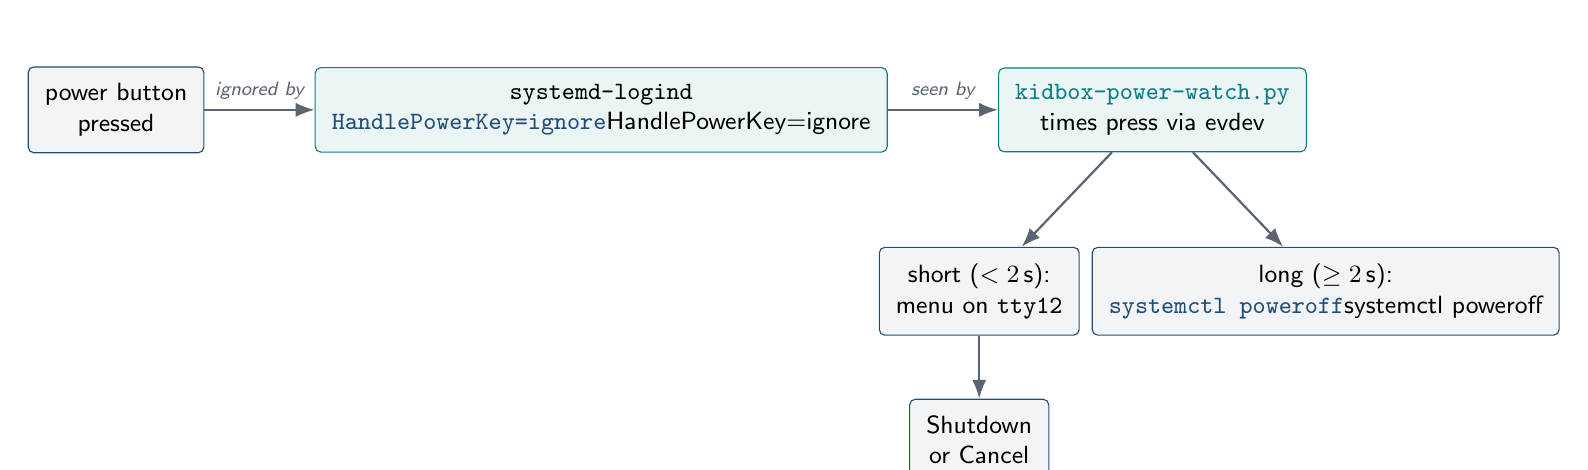
\begin{tikzpicture}[node distance=7mm and 14mm]
\node[stage] (press) {power button\\pressed};
\node[accent,right=of press] (logind) {\texttt{systemd-logind}\\\code{HandlePowerKey=ignore}};
\node[accent,right=of logind] (watch) {\file{kidbox-power-watch.py}\\times press via evdev};
\node[stage,below=12mm of watch,xshift=-22mm] (short) {short ($<2$\,s):\\menu on \texttt{tty12}};
\node[stage,below=12mm of watch,xshift=22mm] (long) {long ($\ge2$\,s):\\\code{systemctl poweroff}};
\node[stage,below=8mm of short] (choice) {Shutdown\\or Cancel};

\draw[flow] (press)--node[lbl,above]{ignored by}(logind);
\draw[flow] (logind)--node[lbl,above]{seen by}(watch);
\draw[flow] (watch)--(short);
\draw[flow] (watch)--(long);
\draw[flow] (short)--(choice);
\end{tikzpicture}
\caption{One button press, routed by three cooperating components.}
\label{fig:power}
\end{figure}

\subsection{Part 1: telling logind to stand down}

The file \file{config/systemd/kidbox-power.conf} is installed as a
\emph{drop-in} at \file{/etc/systemd/logind.conf.d/\allowbreak kidbox-power.conf}:

\begin{lstlisting}
[Login]
HandlePowerKey=ignore
# HandlePowerKeyLongPress=poweroff  # systemd >= 245
\end{lstlisting}

\code{HandlePowerKey=ignore} tells logind to do nothing on the power key, ceding
control to kidbox's own watcher. The commented \code{HandlePowerKeyLongPress}
line is a thoughtful note: newer systemd can itself distinguish a long press, but
kidbox can't assume that version, so it handles \emph{both} press lengths in its
own watcher instead.

\begin{deeper}[Going deeper: drop-ins, and why you never edit the original file]
Notice kidbox never edits \file{/etc/systemd/logind.conf} directly. Instead it
drops a small file into a \file{.conf.d/} directory beside it. This is the
pervasive systemd \emph{drop-in} pattern: the main config plus every snippet in
the matching \file{.d/} directory are merged at load time, with later files
overriding earlier keys. The payoff is that package upgrades can replace the
original file freely without clobbering your changes, and your change is a
single self-describing file you can list, version, or delete. The same mechanism
is what \code{systemctl edit getty@tty1} used earlier for autologin --- it just
writes an \file{override.conf} drop-in for you.
\end{deeper}

\subsection{Part 2: watching the button with \texttt{evdev}}

The watcher (\file{bin/kidbox-power-watch.py}) is the clever heart. It reads the
kernel's raw input events directly through \textbf{evdev}. First it finds every
input device that claims to emit a power key:

\begin{lstlisting}[language=python]
for device_path in list_devices():
    device = InputDevice(device_path)
    caps = device.capabilities()
    if ecodes.EV_KEY in caps and ecodes.KEY_POWER in caps[ecodes.EV_KEY]:
        devices.append(device)
\end{lstlisting}

Then it watches \emph{all} of them at once with \code{select.select()} ---
blocking efficiently until any device has an event --- and times the gap between
the key-press (\code{value == 1}) and key-release (\code{value == 0}) events. A
gap of $\geq 2$ seconds is a long press (immediate poweroff); a shorter one
launches the menu. A half-second debounce guards against electrical bounce.

The repository even keeps the throwaway probe script (\file{power.py}) that was
clearly used to \emph{discover} which devices report the power key:

\begin{lstlisting}[language=python]
for d in list_devices():
  dev = InputDevice(d)
  has_power = ecodes.KEY_POWER in dev.capabilities().get(ecodes.EV_KEY, [])
  print(f'{d}: {dev.name} (KEY_POWER={has_power})')
\end{lstlisting}

\begin{deeper}[Going deeper: the Linux input subsystem and \texttt{evdev}]
Every key, button, knob, and touchpad on a Linux machine surfaces through the
\textbf{input subsystem} as a device file under \file{/dev/input/event*}. Reading
one yields a stream of fixed-size \emph{input events}, each a \texttt{(type,
code, value)} triple: type \code{EV\_KEY} for buttons, codes like
\code{KEY\_POWER} (numeric \texttt{116}) for which key, value \code{1}/\code{0}
for press/release (and \code{2} for autorepeat). \texttt{evdev} (``event
device'') is this generic interface, and the Python \texttt{python3-evdev}
package is a thin, pleasant wrapper over it. The reason the watcher monitors
\emph{every} device advertising \code{KEY\_POWER} --- rather than the first one
--- is a hard-won subtlety the code comments record: on real hardware several
virtual devices (an ACPI button, a GPIO button, a PMIC) all \emph{claim} the
capability, but only one actually \emph{fires}. Watching them all and reacting to
whichever speaks is the robust answer, and the git history shows this was learned
the hard way (``Monitor all KEY\_POWER devices instead of just the first'').
\end{deeper}

\begin{deeper}[Going deeper: the road not taken --- \texttt{acpid} and \texttt{udev}]
Before \texttt{systemd-logind}, the canonical way to handle a power button was
\textbf{acpid}, the ACPI event daemon: it listened for ACPI events (lid, power,
sleep) and ran shell scripts from \file{/etc/acpi/events/}. Many embedded
projects still use it. A second alternative is a \textbf{udev} rule that runs a
program when a specific input device appears. kidbox's choice --- a long-running
service reading evdev itself --- is heavier than a udev one-liner but gives it
exactly what it needs: precise press \emph{timing}, which neither acpid's
event-callback model nor a udev rule expresses naturally. It's a good example of
picking the tool whose \emph{shape} matches the problem (``measure a duration'')
rather than the most common one.
\end{deeper}

\subsection{Part 3: the confirmation menu on its own VT}

On a short press the watcher runs \file{bin/kidbox-power-menu.sh}, which does
something delightfully sneaky. The watcher runs as a systemd service with
\emph{no controlling terminal}, but \texttt{whiptail} needs a terminal to draw
on. So the script:

\begin{lstlisting}[language=bash]
export TERM=linux                       # services inherit no TERM
ORIG_VT=$(cat /sys/class/tty/tty0/active | grep -o '[0-9]*$')
chvt 12                                 # jump to an unused VT
exec </dev/tty12 >/dev/tty12 2>&1       # attach all fds to it
whiptail --title "Power Button" --nocancel --menu ... 1 Shutdown 2 Cancel ...
\end{lstlisting}

It records the current VT (so it can return there on Cancel), switches the
display to \texttt{tty12} with \code{chvt}, then \emph{re-attaches its own
standard input, output, and error to \file{/dev/tty12}} so \texttt{whiptail} has
a real terminal to read and draw on. Shutdown runs \code{systemctl poweroff};
Cancel (or Esc) \code{chvt}s back to wherever the child was. Using a dedicated,
otherwise-empty VT means the power dialog and the main menu (on \texttt{tty1})
can never collide for the keyboard --- a genuinely elegant solution to ``two
programs, one keyboard.''

\subsection{The service unit, and what its hardening buys}

The watcher is kept alive by \file{kidbox-power-watch.service}:

\begin{lstlisting}
[Service]
Type=simple
ExecStart=/usr/local/bin/kidbox-power-watch.py
Restart=always
RestartSec=5
ProtectSystem=strict
ProtectHome=yes
PrivateTmp=yes
DevicePolicy=auto
\end{lstlisting}

\code{Restart=always} means systemd revives the watcher if it ever dies ---
essential for something guarding the power button. The rest is
\emph{sandboxing}, and it's worth knowing what each line actually does, because
these directives are systemd's quiet superpower:

\begin{itemize}
\item \code{ProtectSystem=strict} --- mounts the \emph{entire} filesystem
read-only for this process, except \file{/dev}, \file{/proc}, \file{/sys}. The
service literally cannot modify a file anywhere unless explicitly allowed.
\item \code{ProtectHome=yes} --- makes \file{/home} (and \file{/root},
\file{/run/user}) appear \emph{empty} to the process. A power watcher has no
business reading anyone's files, so it can't.
\item \code{PrivateTmp=yes} --- gives the service a private \file{/tmp} that
vanishes when it stops, so it can't be used to leak or stash data.
\item \code{DevicePolicy=auto} --- the device-access policy that still lets it
reach the input devices it genuinely needs.
\end{itemize}

\begin{deeper}[Going deeper: services as lightweight sandboxes]
These directives lean on the same kernel primitives --- mount namespaces,
cgroups, capability dropping --- that containers like Docker are built from.
systemd quietly exposes them one keyword at a time, so an ordinary service can be
locked down to ``can read input devices, can't touch the disk or anyone's home
directory'' without any container runtime at all. For a process that runs as
\texttt{root} (which this one must, to read raw input devices), that defence in
depth is exactly right: if the watcher were ever compromised, the blast radius is
deliberately tiny. You can audit any unit's effective sandboxing with
\texttt{systemd-analyze security kidbox-power-watch.service}, which scores each
setting --- a genuinely fun command to run on your own machine.
\end{deeper}

\begin{fieldnote}
A small drift between docs and code: the README and the unit's own header
comment still describe the menu as ``Shutdown / Reboot / Cancel,'' but the git
history (``Remove reboot option from power menu'') and the current script offer
only \emph{Shutdown} and \emph{Cancel}. The behaviour is the intended one; the
comments just haven't caught up. A one-line edit to the README and the
\file{.service} header would close the gap.
\end{fieldnote}

% ===========================================================================
\section{Permissions: a deliberately small amount of power}

kidbox grants the locked-down \texttt{girls} account exactly one privileged
ability, and does it carefully. The installer writes a \texttt{sudoers} drop-in:

\begin{lstlisting}[language=bash]
SUDOERS_FILE="/etc/sudoers.d/kidbox-shutdown"
cat > "$SUDOERS_FILE" <<EOF
girls ALL=(ALL) NOPASSWD: /sbin/shutdown -h now
EOF
visudo -c -f "$SUDOERS_FILE" || { rm -f "$SUDOERS_FILE"; exit 1; }
chmod 0440 "$SUDOERS_FILE"
\end{lstlisting}

This lets \texttt{girls} run \emph{only} the exact command \code{/sbin/shutdown
-h now}, and only that --- not \code{shutdown} with other arguments, not anything
else --- and without a password (the account has none). The menu's ``Shutdown''
item uses precisely that command.

Three things here are textbook-correct and worth internalising:

\begin{itemize}
\item \textbf{A drop-in, not an edit to \file{/etc/sudoers}.} Same reasoning as
the systemd drop-ins: upgrades and tooling stay clean, and the grant is one
self-contained, removable file.
\item \textbf{\code{visudo -c} validates before activating.} A syntax error in a
live \texttt{sudoers} file can lock \emph{everyone} out of \texttt{sudo}. The
installer validates the file and \emph{deletes it on failure} rather than leave a
broken rule in place. This is the single most important habit in
\texttt{sudoers} editing, and the script gets it right.
\item \textbf{Mode \code{0440}.} \texttt{sudo} refuses to read a
\texttt{sudoers} file that is group- or world-writable (a security check);
\code{0440} (read-only for owner and group, nothing for others) is the required
permission.
\end{itemize}

\begin{deeper}[Going deeper: the threat model is ``a toddler,'' not ``an attacker'']
It's worth being honest about what this security is \emph{for}. The
passwordless account, the inescapable menu, the trapped Ctrl+C --- none of it
would stop a determined teenager with a keyboard and the internet. That's fine,
because the threat model is a five-year-old who might wander into a shell, delete
something, or shut the machine off mid-drawing. kidbox is built to prevent
\emph{accidents and confusion}, not \emph{adversaries}. Recognising which kind of
security you're building is half of doing it well; over-engineering a child's
computer against nation-state attackers would be its own kind of mistake. The
group memberships the installer grants (\texttt{audio}, \texttt{video},
\texttt{input}, \texttt{plugdev}, \texttt{render}) follow the same restraint:
exactly the hardware-access groups a desktop user needs, and nothing like
\texttt{sudo} or \texttt{adm}.
\end{deeper}

% ===========================================================================
\section{Installation: one idempotent shell script}

\file{install.sh} (originally drafted, its header notes, with ChatGPT's help)
turns a stock Raspberry Pi OS into a kidbox. It's a model of how to write an
installer in plain \texttt{bash}, and several of its techniques are reusable far
beyond this project.

\subsection{Safety rails at the top}

\begin{lstlisting}[language=bash]
#!/usr/bin/env bash
set -euo pipefail
[[ $EUID -ne 0 ]] && { echo "Please run as root."; exit 1; }
KID_USER="${KID_USER:-girls}"
\end{lstlisting}

\code{set -euo pipefail} is the ``strict mode'' every serious shell script
should open with: \code{-e} exit on any unhandled error, \code{-u} treat unset
variables as errors (catching typos), \code{pipefail} make a pipeline fail if
\emph{any} stage fails, not just the last. The root check fails fast and
friendly. \code{KID\_USER:-girls} reads an environment variable with a default,
which is why \code{sudo KID\_USER=girls ./install.sh} works.

\subsection{Idempotency: safe to run again and again}

The README tells you to \emph{update} by re-running the installer, so every step
must be safe to repeat. The script achieves this in several ways:

\begin{itemize}
\item It creates the user only \code{if ! id -u "\$KID\_USER"} --- skipping if
present.
\item It uses the \texttt{install(1)} command (not \texttt{cp}) to copy files
with explicit permissions in one atomic step --- e.g.\ \code{install -m 0755} for
scripts, \code{install -m 0644} for data, \code{install -d} to create
directories.
\item For the children's \emph{typing} files it copies \emph{only if the
destination is missing}, so a child's saved text is never clobbered by an update
--- while BASIC and Logo example files \emph{are} overwritten, because they're
templates.
\end{itemize}

\subsection{The marker-block trick for \file{.bash\_profile}}

The most quietly clever part is how the installer edits \file{.bash\_profile}
without ever duplicating its block on re-runs. It wraps its snippet in marker
comments and, before re-adding, strips any previous block with \texttt{awk}:

\begin{lstlisting}[language=bash]
MARK_BEGIN="# >>> kidbox menu autostart >>>"
MARK_END="# <<< kidbox menu autostart <<<"
awk -v b="$MARK_BEGIN" -v e="$MARK_END" '
  $0==b {inblock=1; next}
  $0==e {inblock=0; next}
  !inblock {print}
' "$BASH_PROFILE" > "$tmp"
# ... then append a fresh marked block
\end{lstlisting}

The \texttt{awk} program prints every line \emph{except} those between the
markers, deleting any prior install. Then a fresh block is appended. Run the
installer ten times and you still get exactly one block. If those
``\code{>>>}/\code{<<<}'' markers look familiar, it's because this is the very
same pattern \texttt{conda}, \texttt{nvm}, and countless other tools use to manage
their lines in your shell config --- a small, robust convention worth keeping in
your own toolbox.

\subsection{Then it wires up the system}

The tail of the script installs the systemd units, the sudoers file, and the
logind drop-in we've already met, then \code{systemctl daemon-reload}, enables
and starts the power watcher, and restarts \texttt{systemd-logind} to pick up the
new config. The package list at the top (\code{apt-get install} of \texttt{ucblogo},
\texttt{python3-pcbasic}, \texttt{tuxpaint}, \texttt{xserver-xorg}, \texttt{xinit},
\texttt{matchbox-window-manager}, \texttt{whiptail}, \texttt{xbindkeys},
\texttt{chromium-browser}, \texttt{mpg123}, \texttt{python3-evdev}, and friends) is
the complete bill of materials for everything described in this report.

\begin{deeper}[Going deeper: the road not taken --- configuration management]
A shell installer is the simplest possible answer to ``put these files here and
flip these switches.'' The industrial alternative is a \emph{configuration
management} tool --- Ansible, Puppet, Salt --- where you describe the desired
\emph{end state} (``this file exists with this content and mode; this service is
enabled'') and the tool figures out how to get there, idempotently, by design.
Those tools shine when you manage a hundred machines and need declarative
guarantees. For one Pi in a child's room, a 240-line \texttt{bash} script you can
read top to bottom is not just adequate, it's \emph{more} in keeping with the
project's ``simple and explicit'' creed than a YAML playbook would be. Still,
it's instructive to notice that the script is hand-rolling, in imperative shell,
exactly the idempotency (create-if-missing, copy-if-changed, edit-once) that
Ansible would give you declaratively for free --- a nice lens on what those big
tools are actually \emph{for}.
\end{deeper}

% ===========================================================================
\section{The instruction booklet: LaTeX and a little bookbinding}

The last subsystem is the one you'll physically hold: \file{doc/kidbook.tex}, a
LaTeX document typeset and then \emph{imposed} into a foldable, staplable
booklet. It's a charming corner of the project because it reaches all the way
from digital typesetting into paper craft.

\subsection{A book sized for small hands}

The document class is KOMA-Script's \texttt{scrbook}, with a custom page size:

\begin{lstlisting}
\documentclass[11pt,oneside,paper=5.5in:8.5in,DIV=13,
  chapterprefix=false,headings=big]{scrbook}
\end{lstlisting}

\code{paper=5.5in:8.5in} is \emph{half} of US Letter --- the natural page size
for a booklet folded from letter paper. \code{DIV=13} is KOMA-Script's
\emph{type-area} control: rather than set margins directly, you tell it into how
many strips to divide the page, and it computes classically-proportioned margins
for you. \code{oneside} (versus \texttt{twoside}) keeps margins symmetric, which
matters once the pages are imposed.

\subsection{From PDF to bootable booklet: imposition}

The \file{doc/Makefile} builds two PDFs:

\begin{lstlisting}[language=bash]
pdf: $(TEX).tex
	pdflatex $(TEX).tex
	pdflatex $(TEX).tex            # twice, to resolve the table of contents
booklet: pdf
	pdfjam --booklet true --landscape --paper letterpaper $(PDF) -o $(BOOKLET)
\end{lstlisting}

The first target produces an ordinary, page-1-2-3-4 PDF at half-letter size. The
second runs \texttt{pdfjam} (a wrapper around the \texttt{pdfpages} LaTeX
package) with \code{--booklet}, which performs \textbf{imposition}: it reorders
and 2-up's the pages onto landscape letter sheets so that, when you print
double-sided, fold the stack in half, and staple the spine, the pages come out in
reading order. The README's printing instructions (duplex, long-edge binding,
fold horizontally, staple the fold) are the physical other half of that
algorithm.

\begin{deeper}[Going deeper: signatures, imposition, and why page 1 sits next to the last page]
Imposition is older than computers --- it's how every paperback you own was made.
Fold one sheet of paper in half and you get four pages (two per side); the trick
is that those four pages are \emph{not} 1, 2, 3, 4 in sequence on the flat sheet.
On the outside of a single folded sheet sit page~1 and the \emph{last} page,
back to back with page~2 and the second-to-last. A folded bundle like this is
called a \textbf{signature}, and real books are sewn from many signatures in a
row. This is exactly why the booklet must have a page count that's a multiple of
four (you can even see a commented-out ``repeat until page count is a multiple of
4'' reminder at the end of \file{kidbook.tex}), and why \texttt{pdfjam} has to
compute that surprising 1-next-to-last ordering. The same maths that lays out a
medieval manuscript lays out this Raspberry Pi instruction book.
\end{deeper}

\begin{deeper}[Going deeper: what TeX is, and why we run it twice]
\TeX{}, Donald Knuth's typesetting system from the late 1970s, was born of his
disgust at the typography of his own books' second edition; he decided to fix
typesetting itself and didn't publish the next volume for a decade. \LaTeX{}
(Leslie Lamport, 1980s) is a layer of sensible document-structure macros on top.
The reason the \texttt{Makefile} runs \texttt{pdflatex} \emph{twice} is a famous
\TeX{} quirk: the first pass discovers where every chapter and page lands and
writes those numbers to an auxiliary file; the second pass reads that file back
to build a correct table of contents and cross-references. Complex documents
sometimes need three passes, or the \texttt{latexmk} tool, which simply keeps
running \TeX{} until the auxiliary files stop changing. This very report you're
reading was built the same way.
\end{deeper}

% ===========================================================================
\section{The development story in the repository}

A last, more human layer: the repository itself tells the story of how kidbox
was built, and it matches your description of the work.

The \file{.claude/} directory holds a \file{README.md} that briefs an AI
assistant on the project's philosophy and structure, plus two
\emph{slash-command} definitions --- \file{build-docs} (``run \texttt{make} in
\file{doc/}'') and \file{check-structure} (``verify the key files exist''). These
are little reusable instructions for the assistant, the modern equivalent of a
\texttt{Makefile} target written in English.

The git history is candid and instructive. You can watch the power button
feature being fought into existence over a run of commits --- ``Attempt to get
the power button service to work,'' ``Monitor all KEY\_POWER devices instead of
just the first,'' ``Fix power menu: monitor all devices, use dedicated VT12'' ---
which is precisely the evdev/multi-device lesson documented earlier. There are
honest commits named \texttt{foobar} and \texttt{tmp script}, a ``Fix AI slop;
better way of setting size,'' and a tidy set of merge commits from
\texttt{claude/}-prefixed feature branches. It is a faithful record of
vibe-coding with a careful human steering: each AI-generated lurch followed by a
correcting hand.

\begin{deeper}[Going deeper: ``simple and explicit'' as an engineering discipline]
Step back and the whole project rhymes. Every layer chooses the small, legible,
inspectable option over the powerful, opaque one: a shell installer over Ansible;
\texttt{xinit} over a display manager; \texttt{matchbox} over a desktop
environment; \texttt{whiptail} over a graphical kiosk framework; an evdev script
over a black-box appliance; raw \texttt{sudoers} and systemd drop-ins over some
management layer. Each individual choice is defensible on its own (lighter on the
Pi, fewer dependencies), but together they express a single coherent value: a
machine whose every behaviour can be traced to a file a curious person --- child
or parent --- can open and read. That is the same promise the README makes to its
users, kept by the engineering all the way down. It is, quietly, a rather elegant
piece of work.
\end{deeper}

% ===========================================================================
\section*{Appendix A: File map}
\addcontentsline{toc}{section}{Appendix A: File map}

\begin{table}[ht]
\small
\begin{tabular}{@{}>{\ttfamily}p{0.40\textwidth}p{0.55\textwidth}@{}}
\toprule
\rmfamily\textbf{Path} & \textbf{Role}\\
\midrule
install.sh                  & Idempotent system installer (root).\\
power.py                    & One-off probe: which devices report KEY\_POWER.\\
bin/menu.sh                 & The whiptail main menu loop.\\
bin/clock.sh                & Launches the HTML clock in Chromium kiosk.\\
bin/timer.sh                & Asks minutes (zenity), runs the countdown.\\
bin/timer-countdown.sh      & The per-second countdown + sound.\\
bin/stopwatch.sh            & Count-up timer in a big-font xterm.\\
bin/kidbox-power-watch.py   & evdev power-button watcher (systemd service).\\
bin/kidbox-power-menu.sh    & Power confirmation menu on tty12.\\
config/xinitrc              & Minimal X session (WM, hotkeys, one app).\\
config/Xresources           & Large fonts / DPI for X apps.\\
config/xbindkeysrc          & Ctrl+Alt+Backspace $\to$ kill X (escape hatch).\\
config/bash\_profile\_snippet.sh & Console font + launch menu at login.\\
config/systemd/*            & logind drop-in and the watcher service unit.\\
content/clock.html          & Self-contained analog+digital clock.\\
content/basic/HELLO.BAS     & Starter BASIC program.\\
content/logo/welcome.lg     & Starter Logo procedures.\\
content/typing/*.txt        & Per-child typing files (preserved on update).\\
doc/kidbook.tex             & The instruction booklet source.\\
doc/Makefile                & Builds the half-letter PDF and imposed booklet.\\
\bottomrule
\end{tabular}
\end{table}

\section*{Appendix B: A field guide to the commands and concepts}
\addcontentsline{toc}{section}{Appendix B: Glossary}

\begin{description}[style=nextline,leftmargin=0pt,font=\ttfamily\color{kbblue}]
\item[agetty] The program a \texttt{getty@} service runs to offer a console
login; \code{--autologin} skips authentication.
\item[ALSA / amixer] The kernel sound layer and its command-line mixer.
\item[chvt] Switch the active virtual terminal from the command line.
\item[DPMS] Display Power Management Signaling --- how X tells a monitor to sleep.
\item[drop-in] A small config file in a \texttt{.d/} directory, merged over a
main config; used here for logind, getty, and sudoers.
\item[evdev] The Linux generic input-event interface under
\file{/dev/input/event*}.
\item[getty / tty] ``Get tty''; a tty is a terminal, named for the
teletypewriter.
\item[idempotent] Safe to run repeatedly with the same result --- the installer's
design goal.
\item[imposition] Reordering pages so a folded, stapled stack reads correctly.
\item[matchbox] A minimal window manager for small screens.
\item[NEWT\_COLORS] Environment variable that recolours \texttt{whiptail};
abused here to hide the OK button.
\item[systemd-logind] The systemd service managing login sessions and power keys.
\item[XLFD] X Logical Font Description --- the 14-field hyphenated core-font name.
\item[xinit] Starts an X server plus one client and exits when that client does.
\item[xrdb] Loads the X resource database (\file{.Xresources}).
\end{description}

\vfill
\begin{center}
\small\itshape\color{kbgrey}
End of report. Built with \texttt{pdflatex}; typeset in Bitstream Charter.\\
Sleep well, and may your children never find a shell prompt.
\end{center}

\end{document}
